\documentclass[12pt,a4paper]{article}

\usepackage[T1]{fontenc}
\usepackage[utf8]{inputenc}

\usepackage[english]{babel}
\usepackage{csquotes}

\usepackage[authordate-trad,backend=biber]{biblatex-chicago}
\usepackage{todonotes}
\usepackage{circuitikz}
\usepackage{mathtools}
\addbibresource{jabref.bib}

%opening
\title{By how far have recent churn-reduction techniques improved quality of experience in peer-to-peer video streaming environments?}
\author{Martin Symons}

\begin{document}

\maketitle

\begin{abstract}
abstract !!! 
\end{abstract}

\section{Introduction}
Within the past ten years, video streaming traffic across the internet has exploded. Traditional client-server architectures places a large load on the small portion of nodes controlled by the streaming host, and lead to dramatic infrastructure costs. To combat this, peer-to-peer systems have been proposed that spread usage across the network's collective resources. Starting with Coolstreaming in 2004, these networks became defacto for IPTV streaming, especially pirated streams. With their utility proven, research accelerated, in pace and complexity. Industry, however, did not pick up. Since the shutdown of New Coolstreaming and PPLive in the late 2000's, these newer solutions have seen little real-world usage.

As such, the actual impact of current research on network performance is vague. Still, research since has suggested that churn has a substantial and exponential impact on client quality-of-service (QoS) beyond that which was considered in these original models. This paper investigates several marked improvements over the best-documented benchmark architecture, New Coolstreaming, with particular focus on methods to reduce churn throughout the network. wordsw words words 

\section{Literature Review}
\subsection{Peer-to-Peer Streaming Fundamentals}
In the late 1990's the traditional client-server architecture began to crack, as computer capabilities began to outpace bandwidth growth across the internet. Small clusters of server nodes were expected to take the burden, whilst ample client resources waited idle. BitTorrent allows a swarm of peers to collaborate in file transmission, maximizing global utilization without overwhelming any single node. Peers instead connect to a tracker or query a global DHT, usually \textit{Mainline DHT}, to gather a list of participatory nodes. Targetting the rarest blocks first, data chunks within the swarm are piped directly over UDP node-to-node. As more peers join the network, the overall bandwidth increases, with download speeds following suit.

This approach exploded onto the internet, claiming 35\% of all upstream traffic (\cite{archiveCacheLogicResearch}). It remained in the number one spot for total traffic until recently - finally dethroned in 2024 by video streaming. 

In a file-share network QoS is taken mostly with upload speed, and by extension bandwidth utilization. Any intermediate action from loading a \textit{.torrent} to completion is irrelevant. Video streaming, in contrast, introduces a large number of real-time requirements essential for a good user experience.



Peer-to-peer networks pipe data directly between nodes through a network, contrasted with the traditional client-server architecture seen most often today.  Compared to file-sharing applications, peer-to-peer video networks face several new complexities. In the former, QoS is ruled almost entirely by bandwidth utilization. Users care only that a desired file eventually reaches them; the journey it takes to completion is unimportant.  probably list some examples Video livestreaming, however, introduces new complexities. playoutdeadlines startupdelay end-to-enddelay
one proposed solution was ip multicasting. it was . fucked. s owe don't use it and instead use the various better solutions
\subsection{Performance Heuristics and Churn}
explaining why we use/care about churn vs other characteristics
\subsection{Overlay Structure}
\subsection{Peer Selection Strategies}
\subsection{Chunk Schedulers}
\subsection{Historic Implementations}
We now consider historic implementations of peer-to-peer streaming systems in relation to the above characteristics. Of most relevance to our paper is DONet, commercially branded Coolstreaming (\cite{1498486}). Considered the first of its breed, Coolstreaming \cite{Xie2007} \cite{asdasd} \cite{1498486}
\subsection{Implementation-Specific Improvements}
\section{Methodology}
We aimed to pit three models against each other in various QoS tests \todo{which?} to gather specific numbers on the improvements between each. Initial tests would be run on New Coolstreaming, widely considered the last popular IPTV P2P system and a good benchmark \todo{we probably already explained this in the lit review}. We would then extend this with fitting modular improvements for further measurements. \todo{name some shit} were particular targets, because \todo{blah}. Finally, we expected to implement a monolithic model, \todo{name}, to compare the capacity of incremental improvements versus the design of a single, deeply-coupled architecture.

As a simulation environment, we chose OverSim. Its included churn mechanisms, quick-switching between simplified and realistic underlay models, and complete debugging suite eased the otherwise involved development cycle. Ejecting from OverSim to OMNET++ would also have been trivial, though was never necessary.

Statistics would be presented with the built-in OMNET++ visualization tools.

\todo{needs expansion. we could mention dates?? what do people normally put here}
\section{Implementation}
We based our initial experiments on New Coolstreaming as described in \cite{Li2008}. We quickly ran into problems - whilst the paper describes the stream manager and buffer map exchange in great detail, little time is given to the membership and partnership managers. The upkeep of the \textit{mCache} with incoming peers is unspecified, as is most connection management action related to churning or failing nodes and some key equations to system function. We pushed forward and attempted to fill the blanks ourselves; the final result, whilst technically functional, invariably failed to meet playout across nodes and was in no way correspondent of New Coolstreaming's measured real-world performance.

The New Coolstreaming paper concludes its discussion on the problem modules stating \textit{"these basic modules form the base for the initial Coolstreaming system,"} and that the New Coolstreaming \textit{"has made significant changes in the design of other components."} We thus considered that these modules were holdovers from the older design, implying New Coolstreaming must be built with  DONet/Coolstreaming as groundwork. We thereby set about an implementation of this more primitive design.

The final DONet implementation completed following two weeks of work. This network was similarly not ideal, though the cause was mostly banal - New Coolstreaming strips the buffer, scheduler and related messaging completely, so we saw no need to optimize these components. More worryingly, the partnership manager collapsed quickly under even minimal churn, discussed later in section \todo{SECTIONWHAT}. Still, this constituted enough the groundwork needed to continue.

Returning with wiser eyes, we fcircuitikzound that our architecture did not align at all with the basic modules in New Coolstreaming. \textit{How could this be?} As discussed later in section \todo{SECTION}, DONet has clarity problems of its own when describing parts of other systems, and we noticed that the output of these components - \textit{M}-number exchanging partners ready for video transmission - \textit{did} align with the older model. We therefore treated this as a simple faulty description, and moved on to the design of the stream manager.

The well-specified stream manager came through without a hitch, but placed new constraints on the partnership manager that our already brittle implementation could not bear. We hence designed \textit{Partnerlink}, a relationship algorithm reconciling the high-churn overlay with New Coolstreaming's low-churn subscription requirements and performance at scale. This new algorithm meshed well with the stream manager, and brought our implementation to a close.

The full development process took over a month. We were therefore not able to complete any further models or make any comparisons on QoS benefits.

\section{Results}
jsut offhandedly mentioning that Yes, It Workas Kind Of
\section{Discussion}
\textit{What went wrong?} New Coolstreaming is not unique as an overlay; no features within should prove particularly challenging to implement. In this section, we explore the Coolstreaming family as a whole, and illuminate the many challenges faced in their implementation amiss in the papers themselves.
\subsection{The Coolstreaming Family Tree}
We have so far regarded Coolstreaming as a dyad of the mesh-pull DONet/Coolstreaming and hybrid-push-pull New Coolstreaming, proposed across two papers. The reality is not so simple. Coolstreaming is formed of two models, as described. However, they have been proposed under \textit{four} different names across \textit{four} papers:

\begin{itemize}
	\item As \textit{DONet} and \textit{Coolstreaming}, in \textit{CoolStreaming/DONet: a data-driven overlay network for peer-to-peer live media streaming} \cite{Zhang2005}
	\item As \textit{Coolstreaming}, in \textit{Coolstreaming: Design, Theory, and Practice} \cite{Xie2007}
	\item As \textit{Coolstreaming+}, in \textit{An Empirical Study of the Coolstreaming+ System} \cite{Li2007}
	\item As \textit{"the new Coolstreaming,"} in \textit{Inside the New Coolstreaming: Principles, Measurements and Performance Implications} \cite{Li2008}.
\end{itemize}

Note that the name \textit{Coolstreaming} is intended by this final paper, but \textit{The New Coolstreaming} became the colloquial model name as a result of its title. Only the first paper contains the old model we have discussed as \textit{DONet/Coolstreaming} - the others all specify \textit{New Coolstreaming}, despite the name differences.

The name \textit{Coolstreaming} legally refers both to the older \textit{DONet} model and the newer \textit{New Coolstreaming} model. The confusion that results is obvious. \cite{Kondo2014} describes the \textit{SCAMP} membership protocol, the push-pull mechanism and the bootstrap node as part of the same model, despite \textit{SCAMP} being specific to the mesh-pull \textit{DONet}. \cite{Beraldi2010} makes much the same error. \cite{Lan2011} takes \textit{DONet} as its key example of a buffer-map driven overlay, but ascribes it the synchronization method seen in \textit{New Coolstreaming}. Further examples still can be found of correct prose, but with \cite{Xie2007} being cited in \cite{Zhang2005}'s place, or vice versa.

It is interesting to note that the papers themselves appear to have issues keeping the versions straight:  \cite{Li2008} describes the stream manager and new mCache system as part of the \textit{"initial Coolstreaming system"} and replaced in \textit{"the new Coolstreaming system"}, despite all of these components being local to \textit{New Coolstreaming} only - hence our initial hesitance to visit \textit{DONet}.

This escalates considering the final three papers. \cite{Xie2007} is the canon definition of \textit{New Coolstreaming}, alongside analysis of a real-world test period to determine convergence rates, start-up delay and other overlay-specific statistics. The other papers duplicate this and add further analysis: \cite{Li2007} splits users into categories, identifying network traversal problems and their respective impact on contribution. \cite{Li2008} performs an additional simulation to identify ideal values for key system parameters.

This duplication means each paper opens with a definition of \textit{New Coolstreaming}. These are not summaries - the \textit{Coolstreaming+} specification is shortest yet still clocks in at two and a half pages. The majority of this text is word-for-word identical between papers, or at best reworded. The membership and partnership managers, though, have their specifications cut down completely, no longer parsing as a working system. For instance, connection management is resolved in \cite{Xie2007} by an off-handed mention of TCP - which includes a leaving and timeout mechanism, if specified. In the other papers, TCP is never mentioned; no other connection management is described. Mechanisms to fill the bootstrap node's \textit{mCache} alongside one key function related to playout initialization are similarly constrained to this paper, despite these papers claiming to \textit{"describe the architecture and components in the new Coolstreaming system"}.

Luckily, we appear to be the only researchers to fall into this trap. Resulting development time was certainly extended, but our criticisms of the paper and our final solution remain valid.

\subsection{The Fully-Connected Network Problem}
Both \textit{DONet} and \textit{New Coolstreaming} make the same demands on the partnership manager: given a random partial view of the network, create and maintain at most \textit{M} connections ready for video transmission. Neither paper provides any exact information on how this should be done.

Suppose a node \textit{n} joins a network of size \textit{M + 1}. All existing nodes in the network are fully saturated with partner count \textit{M}. How can this node join the network?

\begin{figure}[!ht]
	\centering
	\resizebox{0.35\textwidth}{!}{%
		\begin{circuitikz}
			\tikzstyle{every node}=[font=\LARGE]
			\draw  (7.5,15) circle (0.75cm) node {\LARGE 4} ;
			\draw  (10,15) circle (0.75cm) node {\LARGE 4} ;
			\draw  (8.75,10) circle (0.75cm) node {\LARGE 4} ;
			\draw  (6.25,12.5) circle (0.75cm) node {\LARGE 4} ;
			\draw  (11.25,12.5) circle (0.75cm) node {\LARGE 4} ;
			\draw [short] (8.25,10.5) -- (6.75,12);
			\draw [short] (9.25,10.5) -- (10.75,12);
			\draw [short] (11,13.25) -- (10.5,14.5);
			\draw [short] (6.5,13.25) -- (7,14.5);
			\draw [short] (8.25,15) -- (9.25,15);
			\draw [short] (8.5,10.75) -- (7.75,14.25);
			\draw [short] (9,10.75) -- (9.75,14.25);
			\draw [short] (7,12.5) -- (10.5,12.5);
			\draw [short] (8,14.5) -- (10.75,13);
			\draw [short] (9.5,14.5) -- (6.75,13);
			\draw  (8.75,18.75) circle (0.75cm) node {\LARGE n} ;
			\draw [dashed] (8.5,18) -- (7.75,15.75)node[pos=0.5,fill=white]{?};
			\draw [dashed] (9,18) -- (9.75,15.75)node[pos=0.5,fill=white]{?};
			\node [font=\LARGE] at (12.5,19.25) {M = 4};
		\end{circuitikz}
	}%
	\caption{Node \textit{n} cannot easily join this fully-connected network.}
	\label{some label}
\end{figure}

In our early \textit{DONet} implementation, we forced nodes to accept all incoming partnerships, removing an old partnership to make room. This created long chains of dropped-and-replaced partnerships before the overlay settled and worsened the impact radius of churn. The move to \textit{New Coolstreaming} came with the demand to maximize partnership lifetimes, as churn would interfere with the push mechanism and result in wasted blocks being sent to a peer, totally invalidating this approach.

Several solutions exist, though none are trivial. Our final implementation requests a node to break one partnership, placing the new partner in the middle. This has a great number of implications on the network, most notably that \textit{M} must now be divisible by 2. Since \textit{DONet} uses \textit{M = 15} as example, this cannot be the implementation as intended by the original authors.

\begin{figure}[!ht]
	\centering
	\resizebox{0.35\textwidth}{!}{%
		\begin{circuitikz}
			\tikzstyle{every node}=[font=\LARGE]
			\draw  (7.5,15) circle (0.75cm) node {\LARGE 4} ;
			\draw  (10,15) circle (0.75cm) node {\LARGE 4} ;
			\draw  (8.75,10) circle (0.75cm) node {\LARGE 4} ;
			\draw  (6.25,12.5) circle (0.75cm) node {\LARGE 4} ;
			\draw  (11.25,12.5) circle (0.75cm) node {\LARGE 4} ;
			\draw [short] (9.25,10.5) -- (10.75,12);
			\draw [short] (11,13.25) -- (10.5,14.5);
			\draw [short] (6.5,13.25) -- (7,14.5);
			\draw [short] (8.5,10.75) -- (7.75,14.25);
			\draw [short] (9,10.75) -- (9.75,14.25);
			\draw [short] (7,12.5) -- (10.5,12.5);
			\draw [short] (8,14.5) -- (10.75,13);
			\draw [short] (9.5,14.5) -- (6.75,13);
			\draw  (8.75,18.75) circle (0.75cm) node {\LARGE 4} ;
			\node [font=\LARGE] at (12.5,19.25) {M = 4};
			\draw [short] (7.5,15.75) -- (8.5,18);
			\draw [short] (10,15.75) -- (9,18);
			\draw [short] (8,18.75) .. controls (5.75,17.75) and (4.75,15.5) .. (6,13.25);
			\draw [short] (8,10) .. controls (2.75,11.5) and (2.5,17.25) .. (8,18.75);
		\end{circuitikz}
	}%
	\caption{A solved topology, as according to the pairing method.}
	\label{some label}
\end{figure}

We can at least infer some details from \textit{DONet}. The \textit{mCache} data structure includes \textit{num\_partners} for each visible node, which is updated but never apparently used. In a healthy network, the likelihood of a node directly knowing another node with less than \textit{M} partners is low. Instead, we assume this to be part of a gossiping mechanism where a gossiped partnership request is directed towards nodes with missing partners, which would also justify the use of \textit{SCAMP} as opposed to a more standard partial view aggregator. We include a similar strategy as part of our implementation; we discuss this in detail later in section \todo{SECTIONNAME}.

That said, the phrasing of the scheduled switching as established \textit{"with nodes randomly selected from [the] mCache"} implies a more direct communication. In this case, it is unknown how \textit{DONet} or \textit{New Coolstreaming} solve this problem.

\subsection{Choosing New Partners}
The two inequalities measuring connection quality are also applied to any candidate partners following a detected failure. Inequality 1 limits the gap between a node's  buffers and the parent's. If we apply this to candidates after failing because of this inequality, we will filter out any nodes further ahead than our old node, slipping further back in our buffer. Assuming we never change our playout position, this new node will not be able to service our entire buffer area.

Furthermore, the nodes seen within this inequality will mostly be those similarly falling behind the swarm; that is, nodes with equally poor connections. This groups poorly performant nodes and drags them backwards across the buffers, eventually collapsing entirely. In our model we disabled inequality 1 when measuring candidates, and performance resumed - \textit{New Coolstreaming} must use some other unspecified mechanism to avoid this.

\subsection{Requesting the Block}
\textit{New Coolstreaming} specifies an algorithm to compare all buffer maps from a node's first partners and calculate the initial block to request. The method through which this is done is somewhat obscure - the subscription map only communicates on-off booleans. We assume this is achieved by manipulating the latest blocks shown to each node to suggest the node has already received up to that block, despite having just joined. This requires some careful planning to execute without triggering subscriptions from nodes but is a clever usage of the limited data structure at play.

A feature unmentioned here is the behaviour-of and restrictions-on the playout index. Neither \textit{Coolstreaming} implementation specifies a recovery mechanism - nodes are assumed to never fall completely behind the swarm. This leaves us two options - either the playout index must never buffer or pause after sync, and continue to play forward on encounter with missing blocks, or the recovery mechanism is left undefined. Given that there is a startup delay listed amongst the results, we can assume the latter. If the stream does include buffering or the node is suffering poor local performance, though, the need to recover is inevitable. There are many options for approach that impact performance, and one best solution should ideally be provided.

\subsection{Production Optimizations}
\textit{DONet} defers to \textit{SCAMP} for membership connection management, \todo{we need to establish ahead of time the fanout proofs of SCAMP etc.} before overruling it on several counts. Where \textit{SCAMP} automatically adjusts membership count in sync with the size of the system, \textit{DONet} enforces a hard limit of \textit{M} nodes, usually 15. The indirection mechanism is implemented only in primitive form, with only nodes within the origin's view being available as contacts. As \textit{DONet} only uses \textit{SCAMP} to gather a random partial view, and does not use it as a means of message transmission itself, \textit{DONet} does not require \textit{SCAMP}'s full set of guarantees. Whilst we have not been able to perform experiments to prove this, we hypothesize that these restrictions therefore make no negative impact on the network, included to reduce message overhead.

Other optimizations are less successful. \textit{SCAMP} specifies a leasing system to remove dead nodes from the pool, which \textit{DONet} accepts. However, in the case that the partnership manager finds a partner that fails to send a buffer map in a given period, the partnership overrides the membership manager to remove the node from the \textit{mCache}. The partnership manager then emits a departure message on its behalf, which is gossiped \textit{"similarly to the membership message,"} i.e. once to a peer who then repeats it to every node in its \textit{mCache}. Since exactly \textit{M} departure messages are gossiped, every message would have to reach a peer knowing the failed node for a clean exit. The layers of indirections involved in membership management, however, make it unlikely for this message to reach any such peer at all.

This mechanism is applied even to departure messages sent by a leaving node itself. \textit{SCAMP} notes that each node knows the peers it is subscribed to through its \textit{InView} list - thus, the only requirement for a clean exit is to send a departure to each node it contains. The gossiped alternative makes no gain in message overhead whilst almost totally invalidating its effect on network topology.

This appears to be a malformed optimization to allow nodes to depart each other in case of failure. Even if this were successful, the already-established leasing system means any performance gain would be negligible.

Successful or not, these changes represent a problem: we fall back to some existing research solution for a problem and then brain slug \todo{is this actually a good turn of phrase} it for some slight gain, in the process tampering with that solution's proven performance. This is convenient for the original researcher, but requires careful cross-referencing of the two papers for accurate reproduction. New implementation of the model therefore becomes strenuous, and inaccuracies made much more likely.

\subsection{What does Coolstreaming need to be?}
The \textit{Coolstreaming} family has been replaced. Production networks today will prefer to use monolithic solutions like \todo{mention wiotadiof}. \textit{Coolstreaming}'s usage now lies entirely in the research domain - used as a base for reproducible results, a testbed for new modular features or a shared point of comparison between larger monolithic models. In all of these cases, consistency and ease of development take priority over QoS performance.

The issues mentioned so far are a sign that \textit{Coolstreaming} was never designed for this purpose. \textit{Coolstreaming} aimed to be the leading production overlay of its time, including optimizations that were inconvenient but deemed worth the miniscule performance boost. More than this, \textit{Coolstreaming} was developed as a commercial system first and a research paper second. This may explain the missing features or heavy modifications of existing solutions - the system was still under active maintenance as the papers were written, and so work had to be quick moreso than correct.

In the next section, we introduce a new model to the \textit{Coolstreaming} family designed for research purposes, outlining our priorities and rationale in doing so.

\section{Introducing \textit{coolstreaming-spiked}}
\textit{coolstreaming-spiked} is a new iteration of \textit{Coolstreaming} bringing the two models into synthesis. Research usage is targeted through an easier implementation, thorough central specification and compatibility with a wide range of IPTV improvements. Specifically:

\begin{itemize}
	\item The SCAMP protocol is retained for backwards compatibility with research performed on the original \textit{DONet}.
	\item The partnership connection algorithm is solved and documented as \textit{Partnerlink}, a novel approach providing realistic performance and absolutely minimal churn impact for networks of any scale.
	\item Production optimizations are stripped back to focus on a smaller scope.
	\item Other fixes, such as the disabling of inequality 1 on candidates, are implemented as standard.
\end{itemize}

We now proceed to describe the function of this model.

\subsection{Architecture}
Our component architecture is identical to that seen in \textit{New Coolstreaming}: a membership manager provides the model with a continuous pool of random nodes. The partnership manager filters these nodes to find connections suited for video transmission, and handles the exchange of buffer maps. The stream manager creates parent-child relationships, owns the buffer and forwards blocks to peers. Each node within the architecture is provided a unique \textit{NodeID} - an IP address will suffice.

We incorporate the substream system as defined in \textit{New Coolstreaming}. The video sequence is split into blocks of equal size each assigned a timestamp sequence number. These are shared equally between \(K\)-number zero-indexed substreams, where the \textit{i}-th substream contains blocks with sequence numbers \((nK + \textit{i})\) where \(n\) is a positive integer from zero to infinity. For instance, assuming \(K = 4\), substream 2 would contain blocks with ID \(\{2, 6, 10, 14, ...\}\).

\subsection{Membership Manager}
The membership manager makes the initial contact to an origin node. We then subscribe as members to a subset of nodes using SCAMP to provide the partial view. No changes are made to SCAMP - the standard subscription, unsubscription, indirection, leasing and recovery methods all apply. There is no limit on the size of the \textit{mCache}. The partnership manager can no longer directly influence the mCache or send unsubscription messages on behalf of another node. These changes allow researchers to follow a well-specified, battle-tested paper for gossiping support without cross-referencing our own. The main output of this component is an arbitrarily sized set of random nodes across the network.

In the case that the node ever becomes completely isolated and can no longer aggregate members, the node should recontact the origin and gossip a fresh subscription message.

\subsection{Partnership Manager and \textit{Partnerlink}}
The partnership manager takes these nodes and begins to form TCP connections ready for block transmission. TCP performs the majority of connection upkeep on our behalf - if the connection ends, times out or fails, the partnership should be considered \textit{failed}.

The buffer map system remains as specified in \textit{New Coolstreaming}. Each node regularly emits a buffer map to every partner. A buffer map comprises two tuples of length \textit{K} - the first listing the highest block sequence number received in each substream, the second listing the subscription of substreams to the receiving partner. For instance, a node receiving tuples of \(\{40, 41, 42, 39\}\) and \(\{0, 0, 0, 1\}\) from a partner should infer the node to have most recently received block 39 on substream 3, and prepare a subscription for the node on that substream according to the subscription map. We also transfer a \textit{NodeID} representing an \textit{associated peer} and the node's current \textit{panic status}, discussed later in \todo{section??}. If a partner does not transfer a buffer map in some specified length of time, the partner is missing and the partnership should be considered \textit{failed}.

An exception on valid buffer map syntax is made for when the node has just entered the network. Once buffer maps have been exchanged with some minimum proportion of partners, the node must calculate an ideal starting index based on set of known latest received blocks. Designating \(H_{{S_i},A}\) as the latest block received block for substream \(S_i\) at node \(A\), the starting index at substream \(i\) is calculated as \[I_{S_i} = max\{H_{{S_i},q} : q \in partners\} - T_p\] where \(T_p\) is a constant to be introduced later in section \todo{SECTION NAME}. When pushing buffer maps to partners, a new node should fill its latest block tuple with some exceptional value, either a manually-filtered \textit{null} or a very large negative number to ensure the node is never selected, unless the node intends to make its first subscription on a substream to that node. In this case, the latest block on this substream should be listed as \(I_{S_i} - K\) to ensure the partner's stream manager begins transmission from the relevant point.

\subsubsection{\textit{Partnerlink} Description}
We now describe the \textit{Partnerlink} algorithm. We first make two constraints on the system - a maximum number of partners at each node \(M\) is introduced, where \(M\mod{2} = 0\). Our base join operation grants a node two links per request, so an even partner cap is essential. We define a starting network as two or more nodes in a valid system topology, since at least two peers are necessary to begin splitting. This basic network could be comprised of two guaranteed-trustworthy origin nodes, or built cooperatively with potentially-malicious client nodes.

\tikzset{every picture/.style={line width=0.75pt}} %set default line width to 0.75pt        

\begin{figure}[!ht]
	\centering
	\resizebox{0.25\textwidth}{!}{%
		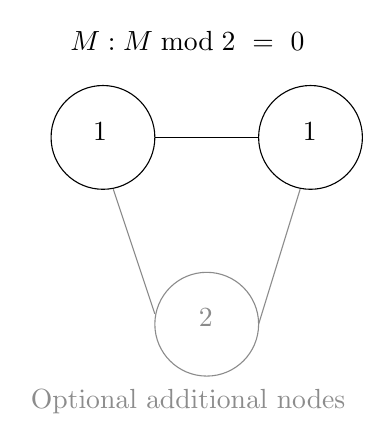
\begin{tikzpicture}[x=0.75pt,y=0.75pt,yscale=-1,xscale=1]
			%uncomment if require: \path (0,224); %set diagram left start at 0, and has height of 224
			
			%Shape: Circle [id:dp8053367545608073] 
			\draw   (360,75) .. controls (360,61.19) and (371.19,50) .. (385,50) .. controls (398.81,50) and (410,61.19) .. (410,75) .. controls (410,88.81) and (398.81,100) .. (385,100) .. controls (371.19,100) and (360,88.81) .. (360,75) -- cycle ;
			%Shape: Circle [id:dp5139832099367154] 
			\draw   (260,75) .. controls (260,61.19) and (271.19,50) .. (285,50) .. controls (298.81,50) and (310,61.19) .. (310,75) .. controls (310,88.81) and (298.81,100) .. (285,100) .. controls (271.19,100) and (260,88.81) .. (260,75) -- cycle ;
			%Straight Lines [id:da34739028917979153] 
			\draw    (310,75) -- (360,75) ;
			%Shape: Circle [id:dp7166484753359771] 
			\draw  [color={rgb, 255:red, 139; green, 139; blue, 139 }  ,draw opacity=1 ] (310,165) .. controls (310,151.19) and (321.19,140) .. (335,140) .. controls (348.81,140) and (360,151.19) .. (360,165) .. controls (360,178.81) and (348.81,190) .. (335,190) .. controls (321.19,190) and (310,178.81) .. (310,165) -- cycle ;
			%Straight Lines [id:da740820997595583] 
			\draw [color={rgb, 255:red, 139; green, 139; blue, 139 }  ,draw opacity=1 ]   (290,100) -- (310,160) ;
			%Straight Lines [id:da5098257307652958] 
			\draw [color={rgb, 255:red, 139; green, 139; blue, 139 }  ,draw opacity=1 ]   (380,100) -- (371.33,128.18) -- (360,165) ;
			
			% Text Node
			\draw (268,22.4) node [anchor=north west][inner sep=0.75pt]    {$M:M\bmod 2\ =\ 0$};
			% Text Node
			\draw (279,66.4) node [anchor=north west][inner sep=0.75pt]    {$1$};
			% Text Node
			\draw (380,66.4) node [anchor=north west][inner sep=0.75pt]    {$1$};
			% Text Node
			\draw (330,156.4) node [anchor=north west][inner sep=0.75pt]  [color={rgb, 255:red, 139; green, 139; blue, 139 }  ,opacity=1 ]  {$2$};
			% Text Node
			\draw (249,195) node [anchor=north west][inner sep=0.75pt]   [align=left] {\textcolor[rgb]{0.55,0.55,0.55}{Optional additional nodes}};
			
			
		\end{tikzpicture}
	}%
	\caption{The base topology from which \textit{Partnerlink} must operate.}
	\label{some label}
\end{figure}

Each node tracks an additional set of variables. We maintain a set of \textit{locks} against \textit{NodeID}s for which operations are still in progress, to protect the system when a node receives several requests regarding the same node. We also maintain an \textit{anticipated} partner count \(M_c\), tracking what our partner count will become if all ongoing operations resolve successfully. Making decisions against this value rather than our actual partner count ensures we do not accidentally request partners above our hard limit \(M\).

\textit{Partnerlink} operations can be split into three categories:
\begin{itemize}
	\item \textbf{Initiation}, allowing a healthy node to create new connections with known nodes.
	\item \textbf{Management}, allowing the overlay to adapt after a failed partnership.
	\item \textbf{Panic}, allowing an unhealthy node to recover back to \(M\) connections.
\end{itemize}
We now discuss the systems and messages in place to allow for these operations.

\subsubsection{\textit{Partnerlink} Initiation}
A node \(n\) entering the network for the first time initializes with \(M_c = M\), locking and retrieving \(M / 2\) nodes from its \textit{mCache} and sending a \textit{Split} message to each. This performs the split operation discussed prior, attempting to place the node in-between an existing partnership. The receiving node \(a\) checks that no partnership nor lock is held against \(n\) - if not, the node forwards a \textit{TrySplit} message to a random unlocked partner \(b\), holding locks against it and \(n\). Node \(b\) performs the same checks, also checking that node \(a\) is not locked. If the checks pass, it returns a \textit{TrySplitSuccess} message, breaks the connection with its old partner and initiates with the new node. Node \(a\) receiving a \textit{TrySplitSuccess} breaks the connection similarly and unlocks the two nodes, after which the exchange is complete. The newly joined node has now gained two links, breaking only one in the process. If all messages respond successfully, the node will have created exactly \(M\) partnerships.

If node \(b\) fails its checks, it responds a \textit{TrySplitFailure}. If node \(a\) receives a \textit{TrySplitFailure}, fails its own checks or does not know another unlocked partner, a \textit{SplitFailure} is forwarded back to the new node \(n\) which reduces \(M_c\) by 2 and unlocks the contacted node. This causes the node to immediately begin panicking.

This mechanism was hypothesized to be similar to the existing \textit{DONet} partnership mechanism, and so its performance should be comparable for research purposes.

\subsubsection{\textit{Partnerlink} Panicking}
If a node does not satisfy \(M_c = M\), it is described as \textit{panicking}. We begin to look for alternative ways to create new links in the system.

If \(M_c = M - 1\), we cannot fill our empty partners by splitting, as we would breach our limit. We instead gossip a 
\textit{Panic} message containing our \textit{NodeID} to a random partner. This message is directed across the network towards panicking nodes with priority, as determined from their buffer maps. Otherwise, the message is directed towards any node that is not the original panicking node or the last hop. Otherwise, the message is directed anywhere, or else dropped. If a panicking node receives a \textit{Panic} message, it initiates a connection with the contained node and increases its \(M_c\) by 1. The original node receiving this connection does the same, unless has since stopped panicking, in which case it rejects the connection.

This joins two panicking nodes together directly and grants one new link each. This is mostly effective in very small networks, where nodes impacted by an improper exit are very few hops together. As networks grow and stabilize, the hops between panicking nodes will increase, worsening delay before node recovery. Note that locks do not influence the transmission of this message, as its result on a partner does not influence a node's local link count.

If \(M_c = M - 2\), we fall back to the splitting method. We gossip a \textit{PanicSplit} message containing our \textit{NodeID} to a random partner. This message contains a field \textit{LastHopOpinion}, initialized to \textit{CANT\_HELP}. The same direction mechanism is applied, although with priority now given to non-panicking nodes and a ban on gossiping to locked partners. At each hop, the node performs similar checks as in a regular \textit{Split} - that we are not already partnered with nor hold any locks against the contained node. If the checks pass, the message is gossiped with a \textit{LastHopOpinion} \textit{CAN\_HELP}; else, it is marked \textit{CANT\_HELP}. If these checks pass and the received message was marked \textit{CAN\_HELP}, we perform an additional check if we hold a lock against the last hop node. If we do, the prior mechanism applies. If not, we proceed as if from a successful \textit{TrySplit} - a \textit{PanicSplitSuccess} is gossiped back to the last hop, our partnership with it is closed and a new connection is initiated with the contained node. The node receiving the \textit{Success} message switches connections similarly.

This finds two relatively stable nodes within the network and places the panicking node between them. This is mostly effective in large networks, where the gossiped message will quickly find its way to nodes with no knowledge of the sender. In networks with node count \(Nc \leq M + 1\), this message will never resolve. The resolution rate quickly improves from there.

If \(0 < M_c \leq M - 3\), we gossip both of the above messages at once.

If \(M_c = 0\), we should assume major disturbance amongst our membership peers. The standard SCAMP leave procedure should be followed to cleanly disconnect from the membership network in the membership manager, before recontacting the origin to gather a fresh partial view and begin new partnerships from scratch.

Each of the above messages contains a time-to-live which is checked at each receiving node. If this timeout expires, the message is dropped. It is the responsibility of each panicking node to resend messages after they time out.

These messages are gossiped to partners, though they could instead be gossiped to members. We suspect that gossiping to partners will bias recipients towards those with a larger number of partnerships (i.e. those with more stable connections) allowing for more effective recovery, whereas the \textit{mCache} may contain a greater concentration of already-poor connections. We cannot provide any proof of this theory, however - this would prove a fruitful future research question.

\todo{we need to check this and ensure this is all we ned to toalk about here}
\todo{we forgot about M\_c changes halfway thorugh this}

\subsubsection{\textit{Partnerlink} Leaving}
To avoid unneeded panics when disconnecting a node, it is intuitive to pair nodes back together, undoing the splitting we performed to enter. If we perform this via messaging, however, failing nodes will still panic all of their nodes, adding \(M\) panicking nodes to the network - a substantial overlay breakdown. Instead, we continually inform nodes of their \textit{associated peer} when exchanging buffer maps. A clean leave then commands nodes to switch connections to the node they have already been informed of, and nodes detecting timeouts or a failing node can switch automatically without external assistance. This mechanism allows for overlay repair without any gossiped messages in most cases.

Nodes should be associated deterministically - that is, for as long as a node holds the same partners, the associated peer for each partner should not change. Given a set of partners \{A, B, C, ...\}, the associated peer for A is B, and for B is A. If there is an odd number of partners, the final peer is associated with an exceptional \textit{NodeID} to be caught later. Peers receiving a buffer map should store the new associated peer corresponding to this partnership, replacing any prior peer. If the partnership fails or times out, the node should first attempt to connect to their associated peer. If this connection fails, or the node was associated with the exceptional \textit{NodeID}, the node should reduce \(M_c\) by 1, entering a panic state.

A leaving node should send a \textit{Leave} message to each of its peers before ending the connection. Each receiving node should then immediately attempt the above procedure regardless of the state of the partnership.

\subsubsection{\textit{Partnerlink} Switching}
\textit{coolstreaming-spiked} is designed for compatibility with both \textit{DONet} and \textit{New Coolstreaming} research models. To provide this support, we maintain the switching system unique to \textit{DONet}. At a set interval, each node should perform a standard \textit{Switch} procedure on a random node in its \textit{mCache}, without changing \(M_c\). Two unlocked associated partners should also be locked. If both new links are successful, these two partners should be sent \textit{Leave} messages, so that they reconnect to each other; else, the procedure is abandoned and the two partners unlocked.

\subsection{Stream Manager}


\section{Conclusion}
holy fuck. this sucks

\printbibliography
\end{document}
